\documentclass[12pt]{article}
\usepackage[top=1in, bottom=1in, left=0.75in, right=1.00in]{geometry}

\usepackage{graphicx,color,enumerate,multicol}
\usepackage{amsmath,amsthm,amsbsy,enumitem}
\usepackage{palatino}

%% Setup aproblem environment, 
%% aproblem items
%% subproblems environment
%% subproblem items
\makeatletter
\newcounter{probcount}
\newcounter{subprobcount}
\newlength\probsep
\newlength\pshrinking
\newif\iffirstprob
\newenvironment{aproblems}%
  {\ifhmode\unskip\par\fi\setcounter{probcount}{0}\probsep\parskip
  \sbox\@tempboxa{\textbf{9.}}\pshrinking\wd\@tempboxa\advance\pshrinking\labelsep
  \let\hproblem\aproblem
  \advance\linewidth -\pshrinking
  \advance\@totalleftmargin\pshrinking
  \advance\leftskip\pshrinking}%
  {\ifhmode\unskip \par\fi\advance\leftskip-\pshrinking}%

\newcommand{\aproblem}{%
  \setcounter{subprobcount}{0}%
  \stepcounter{probcount}%
  \def\@currentlabel{\arabic{probcount}}%
  \ifhmode
    \unskip \par
  \fi
%  \addpenalty{-4000}%
  \iffirstprob\else\addvspace\probsep\fi
  \firstprobfalse
  \hskip -\labelwidth\hskip -\labelsep 
  \hbox to\labelwidth{\hss\textbf{\arabic{probcount}.}}\hskip\labelsep
}%

\newcommand{\subprob}{\item\def\@currentlabel{\arabic{probcount}\alph{\thelistlabel}}}
\newcommand{\skipproblem}{\stepcounter{probcount}}


%% The following commands put defined left and right headers on the top, and a page number
%% on the bottom of all pages beyond page 1
\usepackage{fancyhdr}
\pagestyle{fancy}
\fancyfoot[C]{\ifnum \value{page} > 1\relax\thepage\fi}
\fancyhead[L]{\ifx\@doclabel\@empty\else\@doclabel\fi}
\fancyhead[R]{\ifx\@docdate\@empty\else\@docdate\fi}
\headheight 15pt
\def\doclabel#1{\gdef\@doclabel{#1}}
\def\docdate#1{\gdef\@docdate{#1}}
\makeatother

%% General formatting parameters
\parindent 0pt
\parskip 6pt plus 1pt


\doclabel{Math F251: Section 3.3 (and more) Worksheet}
\docdate{Monday 17 February 2020}


\begin{document}
\renewcommand{\d}{\displaystyle}

\begin{aproblems}
% 3.3 #17
\aproblem  Use the quotient rule and the facts below to show that: \quad $\d \frac{d}{dx} \left(\csc x\right) = - \csc x \cot x$

\vspace{-5mm}
\begin{itemize}[itemsep=-1mm]
\item $\csc x = 1/\sin x$
\item $\cot x = \cos x/\sin x$
\item $(\sin x)' = \cos x$
\end{itemize}
\vfill

\aproblem  Differentiate the functions.
\begin{itemize}
% 3.3 #15
\item[] $\d f(\theta) = \theta \cos \theta \sin \theta$
\vfill
% 3.2 #18
\item[] $\d h(r) = \frac{a e^r}{b+e^r}$
\vfill
% 3.3 #5
\item[] $\d y = \sec \theta \tan \theta$
\vfill
% variation
\item[] $\d f(t) = \frac{\sin t}{3 - 5\cos t}$
\vfill
\end{itemize} 

\newpage
\thispagestyle{empty}
% like 3.3 #35
\aproblem  A mass on a spring vibrates horizontally on a surface with friction, as shown.  Its equation of motion is $\d x(t) = \frac{2 \sin t}{e^t}$, where $t$ is in seconds and $x$ is in inches.

\hfill 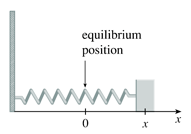
\includegraphics[width=0.3\textwidth]{springslide}

\vspace{-43mm}
\renewcommand{\labelenumi}{(\roman{enumi})}
\begin{enumerate}
\item Find the velocity and acceleration at time $t$.
\vspace{2.0in}

\item Find the position and velocity at time $\d t = \frac{\pi}{2}.$
\vspace{1.8in}

\item Compute $\d \lim_{t\to\infty} x(t)$.
\vspace{1.0in}
\end{enumerate}

% like 3.3 #51
\aproblem  Find the derivative \dots by noticing the pattern:
    $$\frac{d^{79}}{dx^{79}} (\cos x) = \hspace{5.0in}$$
\vfill
\end{aproblems}

\end{document}
